\documentclass{beamer}

\usepackage{amsmath}
\usepackage{amssymb}
\usepackage{amsthm}
\usepackage{amsfonts}

\usepackage{hyperref}

\usepackage{tikz}
\usepackage{color}
\usetikzlibrary{calc,shapes,fadings,automata,backgrounds,petri,shapes,decorations,decorations.pathmorphing,decorations.pathreplacing}


%%%%%%%%%% Tool Names %%%%%%%%%%%%
\newcommand{\pn}{Petri net}
\newcommand{\pns}{Petri nets}
\newcommand{\apical}{$A\pi$-calculus}
\newcommand{\pical}{$\pi$-calculus}
\newcommand{\nest}{\mathit{nest}_\nu}
\newcommand{\depth}{\mathit{depth}}
\newcommand{\set}[1]{\left\{#1\right\}}
\newcommand{\pset}[2]{\set{\,#1\mid#2\,}}
\newcommand{\process}{\mathcal{P}}
\newcommand{\Reach}{\mathit{Reach}}
\newcommand{\subgraph}{\mathrel{\hookrightarrow}}

\newcommand{\tikzMessage}[1]{
  \draw[thick,fill=white] (#1) rectangle ++(0.6, -0.4);
  \path[draw,-,thick] (#1) -- ++(0.3, -0.2) -- ++(0.3, 0.2); 
}
\newcommand{\tikzMessageNode}[2]{
  \node[draw,thick,fill=white,rectangle,inner sep=0pt,minimum height=0.4cm,minimum width=0.6cm] (#1) at (#2) {};
  \path[draw,-,thick] (#2) -- ++(-0.3, 0.2) (#2) -- ++(0.3, 0.2); 
}

\mode<presentation>
{
  \usetheme{Warsaw}
  \useoutertheme{mysplit}
}
% Remove the navigation bar
\setbeamertemplate{navigation symbols}{}

\graphicspath{{./imgs/}}

\title[Analysis of DBP]{Analysis of Depth-Bounded Processes}

\author{Damien Zufferey\inst{1} \and Thomas Wies\inst{2} \and Thomas A.\ Henzinger\inst{1}}
\institute{\inst{1} IST Austria \and \inst{2} New York University}
\date{MSR Redmond, \today}

\begin{document}

% Title
\frame[plain]{\titlepage}

\begin{frame}
  \frametitle{Mobile Processes}

  Why mobile processes ?
  \begin{itemize}
  \item Mobile devices are ubiquitous (e.g. mobile phone).
  \item Mobility becomes common in PL abstraction (e.g. actor model \cite{DBLP:conf/ijcai/HewittBS73}).
  \end{itemize}

  \vspace{10pt}

  Interesting features of mobile processes:
  \begin{itemize}
  \item Process creation
  \item Mobility (communication channels as first class citizens)
  \item Assume no shared memory
  \end{itemize}

  \vspace{10pt}

  How common is mobility ? What are the use cases ?

\end{frame}


\begin{frame}[fragile]
  \frametitle{Example (1): scala/docs/examples/actors/pingpong.scala}

  \begin{columns}
    \column{6cm}
{\tiny
\begin{verbatim}
class Ping(count: Int, pong: Actor) extends Actor {
  def act() {
    var pingsLeft = count - 1
    pong ! Ping
    loop {
      react {
        case Pong =>
          if (pingsLeft % 1000 == 0)
            println("Ping: pong")
          if (pingsLeft > 0) {
            pong ! Ping
            pingsLeft -= 1
          } else {
            println("Ping: stop")
            pong ! Stop
            exit()
          }
      }
    }
  }
}
\end{verbatim}
}

    \column{5cm}
{\tiny
\begin{verbatim}
class Pong extends Actor {
  def act() {
    var pongCount = 0
    loop {
      react {
        case Ping =>
          if (pongCount % 1000 == 0)
            println("Pong: ping "+pongCount)
          sender ! Pong
          pongCount += 1
        case Stop =>
          println("Pong: stop")
          exit()
      }
    }
  }
}
\end{verbatim}
}
  \end{columns}
\end{frame}

\begin{frame}[label=cfa]
  \frametitle{Example (2): scala/docs/examples/actors/pingpong.scala}

  \begin{columns}
    \column{5cm}
    \begin{figure}[!ht]
      \centering
      \textbf{actor$_{ping}$}
      
      \vspace{10pt}
      
      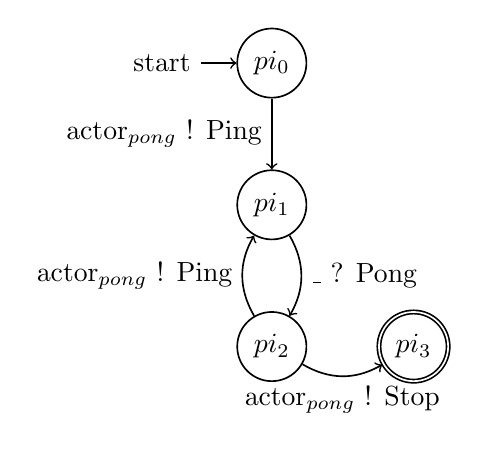
\begin{tikzpicture}[->,auto, node distance=18mm, semithick]
      \node [state,initial] (pi0) {$pi_0$};
      \node [state] (pi1) [below of=pi0] {$pi_1$};
      \node [state] (pi2) [below of=pi1] {$pi_2$};
      \node [state,accepting] (pi3) [right of=pi2] {$pi_3$};
      \path
      (pi0) edge node[left] { actor$_{pong}$ ! Ping } (pi1)
      (pi1) edge [bend left] node[right] { \_ ? Pong } (pi2)
      (pi2) edge [bend left] node[left] { actor$_{pong}$ ! Ping } (pi1)
      (pi2) edge [bend right] node[below] { actor$_{pong}$ ! Stop } (pi3)
      ;
      \end{tikzpicture}
    \end{figure}

    \column{5cm}
    \begin{figure}[!ht]
      \centering
      \textbf{actor$_{pong}$}
      
      \vspace{10pt}
      
      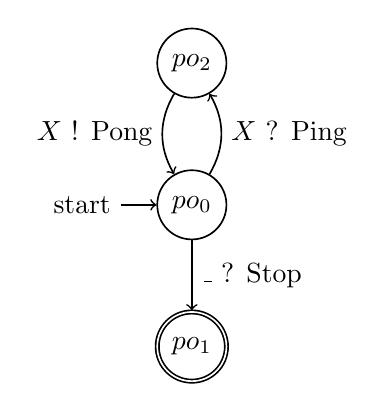
\begin{tikzpicture}[->,auto, node distance=18mm, semithick]
      \node [state,initial] (po0) {$po_0$};
      \node [state,accepting] (po1) [below of=po0] {$po_1$};
      \node [state] (po2) [above of=po0] {$po_2$};
      \path
      (po0) edge node[right] { \_ ? Stop } (po1)
      (po0) edge [bend right] node[right] { $X$ ? Ping } (po2)
      (po2) edge [bend right] node[left] { $X$ ! Pong} (po0)
      ;
      \end{tikzpicture}
    \end{figure}
  \end{columns}
  \begin{itemize}
  \item `?' means receive a message.
  \item `!' means send a message.
  \end{itemize}
\end{frame}


\begin{frame}
  \frametitle{Communication primitives and mobility}

  In the case of the scala actor library:
  
  (asynchronous communication with mailboxes)

  \begin{itemize}
    \item Send the address of an actor to another (within a message).
    \item Messages implicitly carry return address to \texttt{reply}.
    \item \texttt{forward}ing messages.
    \item Creating new process (also a new address and mailbox).
    \item Emulating synch.~communication with shared mailboxes.
  \end{itemize}


\end{frame}

\begin{frame}
  \frametitle{$\pi$-calculus or not ?}

   Shall I introduce the $\pi$-calculus, or can I continue with pictures ?

\end{frame}

\begin{frame}
\frametitle{$A\pi$-calculus: Concepts}

The $\pi$-calculus \cite{DBLP:journals/iandc/MilnerPW92a,DBLP:journals/iandc/MilnerPW92b} is a process calculus able to describe concurrent computations whose configuration may change during the computation.

The \textit{asynchronous} $\pi$-calculus \cite{DBLP:conf/ecoop/HondaT91} is a restriction of the $\pi$-calculus.

\vspace{5pt}
It is build around the notions of 
\begin{description}
\item[Names]: channels as first class values. % also variables: bound
\item[Threads]: concurrent execution of parallel threads: $P\;|\;Q$.
\item[i/o prefixes]: sending/receiving messages.
\end{description}
\end{frame}

\begin{frame}[label=piSyntax]
\frametitle{$A\pi$-calculus: Syntax}
\begin{tabular}{lclr}
$P$ & ::= & $x(y).P $                           & (input prefix)\\
    & $|$ & $\overline{x} \langle y \rangle $   & (output)\\
    & $|$ & $ \sum_i a_i(b_i).P_i $             & (external choice) \\
    & $|$ & $P\;|\;P $                          & (parallel composition)\\
    & $|$ & $!P $                               & (replication) \\
    & $|$ & $(\nu x)P $                         & (name creation)\\
    & $|$ & $0 $                                & (unit process)
\end{tabular}
\end{frame}

\begin{frame}
\frametitle{$A\pi$-calculus: Example (1)}
\begin{columns}

%TODO pong Pong ping Ping
\column{5cm}
\begin{eqnarray*}
pi_0    & = & \overline{\text{pong}_{Ping}}\langle \text{ping}_{Pong} \rangle | pi_1\\
pi_1    & = & \text{ping}_{Pong}().pi_2 \\
pi_2    & = & pi_{2a} \oplus pi_{2b} \\
pi_{2a} & = & \overline{\text{pong}_{Ping}}\langle \text{ping}_{Pong} \rangle | pi_1\\
pi_{2b} & = & \overline{\text{pong}_{Stop}}\langle \rangle | pi_3 \\
pi_3    & = & 0
\end{eqnarray*}

\column{5cm}
\begin{figure}
  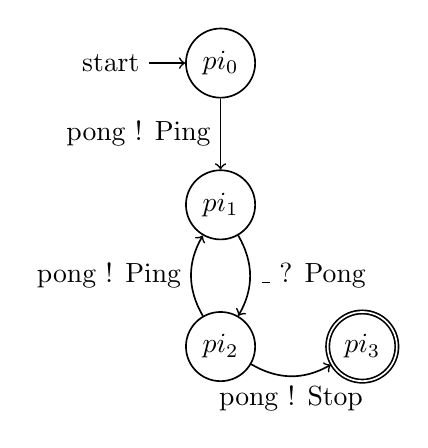
\begin{tikzpicture}[->,auto, node distance=18mm, semithick]
      \node [state,initial] (pi0) {$pi_0$};
      \node [state] (pi1) [below of=pi0] {$pi_1$};
      \node [state] (pi2) [below of=pi1] {$pi_2$};
      \node [state,accepting] (pi3) [right of=pi2] {$pi_3$};
      \path
      (pi0) edge node[left] { pong ! Ping } (pi1)
      (pi1) edge [bend left] node[right] { \_ ? Pong } (pi2)
      (pi2) edge [bend left] node[left] { pong ! Ping } (pi1)
      (pi2) edge [bend right] node[below] { pong ! Stop } (pi3)
      ;
  \end{tikzpicture}
\end{figure}
\end{columns}
\end{frame}


\begin{frame}
\frametitle{$A\pi$-calculus: Example (2)}
\begin{columns}

\column{5cm}
\begin{eqnarray*}
po_0    & = & \text{pong}_{Stop}().po_1 \\
        & + & \text{pong}_{Ping}(X).po_2(X)\\
po_1    & = & 0 \\
po_2(X)    & = & \overline{X}\langle \rangle | po_0
\end{eqnarray*}

\column{5cm}
\begin{figure}
  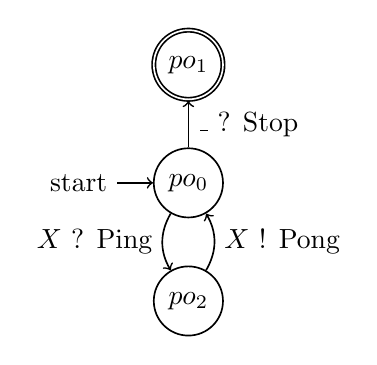
\begin{tikzpicture}[->,auto, node distance=15mm, semithick]
  \node [state,initial] (po0) {$po_0$};
  \node [state,accepting] (po1) [above of=po0] {$po_1$};
  \node [state] (po2) [below of=po0] {$po_2$};
  \path
  (po0) edge node[right] { \_ ? Stop } (po1)
  (po0) edge [bend right] node[left] { $X$ ? Ping } (po2)
  (po2) edge [bend right] node[right] { $X$ ! Pong} (po0)
  ;
  \end{tikzpicture}
\end{figure}
\end{columns}
\end{frame}

\begin{frame}
\frametitle{$A\pi$-calculus: Semantics}
Evaluating a formula in $A\pi$-calculus reduces to applying the rule:


\begin{equation*}
\alt<2>{\textcolor{red}{\overline{a}\langle b \rangle}}{\overline{a}\langle b \rangle} \;|\; \sum_{i \in I} a_i(b_i).Q_i
~~ \rightarrow ~~
\alt<3>{\textcolor{red}{Q_x[b/b_x]}}{Q_x[b/b_x]}
~~~~ \text{where $a_x = a$}
\end{equation*}

\vspace{10pt}

What happens:
\begin{itemize}
\item channel \alt<2>{\textcolor{red}{$a$ carries $b$}}{$a$ carries $b$};
\item $b$ is sent through $a$ and \alt<3>{\textcolor{red}{replace $b_x$ in the continuation $Q_x$}}{replace $b_x$ in the continuation $Q_x$}.
\end{itemize}
\end{frame}


\begin{frame}
  \frametitle{What are Depth-Bounded Processes (DBP) ?}

  \begin{description}
  \item[As buzzwords:]
  concurrent/distributed message-passing programs with process creation and mobility.\\
  (Warning restrictions may apply.)
  \item[For the programmers:] some class of programs using the actor model (Erlang, Scala, Akka, ActorFoundry, $\ldots$)
  \item[For the theoreticians:] a fragment of the $\pi$-calculus.
  \end{description}

\end{frame}


\begin{frame}
  \frametitle{Example: client-server communication pattern}
  \begin{figure}
  \centering
  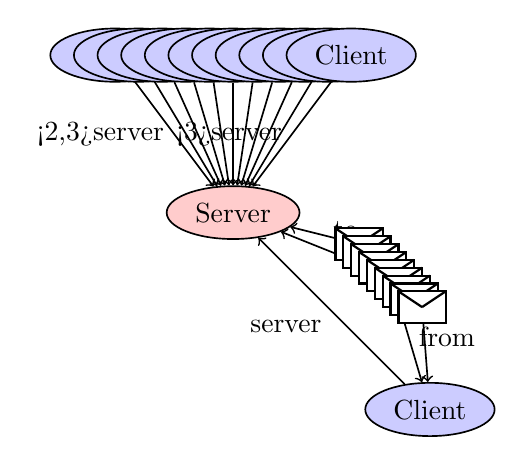
\begin{tikzpicture}[semithick, ->, node distance=2cm]
  \node [draw,ellipse,fill=red!20]  (x) at ( 0, 0) {Server};

  %replication of clients
  \visible<2-> {
  \node [draw,ellipse,fill=blue!20] (ni) at (-1.5, 2) {Client};
  \path  (ni) edge node [left] {\alt<2,3>{server}{}} (x);
  }

  \visible<4-> {
  \node [draw,ellipse,fill=blue!20] (n1) at (-1.2, 2) {Client};
  \path  (n1) edge (x);
  \node [draw,ellipse,fill=blue!20] (n2) at (-0.9, 2) {Client};
  \path  (n2) edge (x);
  \node [draw,ellipse,fill=blue!20] (n3) at (-0.6, 2) {Client};
  \path  (n3) edge (x);
  \node [draw,ellipse,fill=blue!20] (n4) at (-0.3, 2) {Client};
  \path  (n4) edge (x);
  \node [draw,ellipse,fill=blue!20] (n5) at ( 0  , 2) {Client};
  \path  (n5) edge (x);
  \node [draw,ellipse,fill=blue!20] (n6) at ( 0.3, 2) {Client};
  \path  (n6) edge (x);
  \node [draw,ellipse,fill=blue!20] (n7) at ( 0.6, 2) {Client};
  \path  (n7) edge (x);
  \node [draw,ellipse,fill=blue!20] (n8) at ( 0.9, 2) {Client};
  \path  (n8) edge (x);
  \node [draw,ellipse,fill=blue!20] (n9) at ( 1.2, 2) {Client};
  \path  (n9) edge (x);
  }

  \visible<3-> {
  \node [draw,ellipse,fill=blue!20] (nj) at ( 1.5, 2) {Client};
  \path  (nj) edge node [left] {\alt<3>{server}{}} (x);
  }
  
  %replication of messages
  \visible<5-> {
  \node [draw,ellipse,fill=blue!20] (m) at ( 2.5, -2.5) {Client};
  \path  (m) edge node [below left] {server} (x);
  }
  
  \visible<6> {
  \tikzMessageNode{mm}{2.0,-0.8}
  \path  (mm) edge node [right] {from} (m);
  \path  (mm) edge node [above right] {to} (x);
  }

  \visible<7-> {
  \tikzMessageNode{m1}{1.6,-0.4}
  \tikzMessageNode{m3}{1.7,-0.5}
  \tikzMessageNode{m4}{1.8,-0.6}
  \tikzMessageNode{m5}{1.9,-0.7}
  \tikzMessageNode{m6}{2.0,-0.8}
  \tikzMessageNode{m7}{2.1,-0.9}
  \tikzMessageNode{m8}{2.2,-1.0}
  \tikzMessageNode{m9}{2.3,-1.1}
  \tikzMessageNode{m2}{2.4,-1.2}
  \path  (m2) edge (m);
  \path  (m1) edge (x);
  }

  \end{tikzpicture}
  \end{figure}
\end{frame}

\begin{frame}
  \frametitle{What kind of properties are we looking at ?}
  Safety properties, more precisely the control-state reachability problem (aka covering problem).

  \begin{figure}
  \centering
  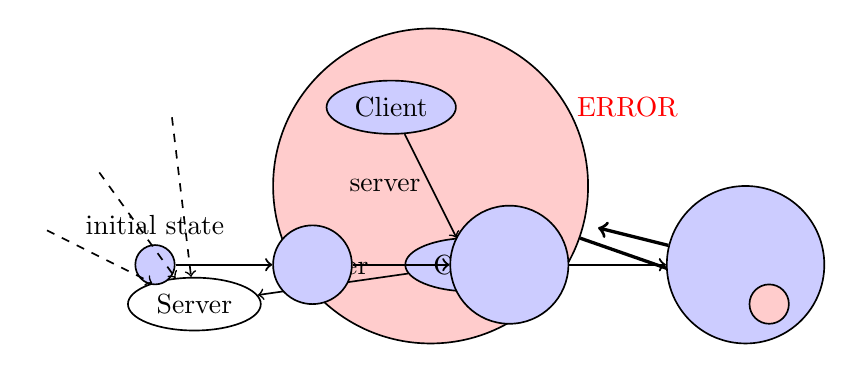
\begin{tikzpicture}[semithick, ->, node distance=2cm]

  \visible<1-2,8> {
  \node[draw,circle,fill=red!20, minimum height=4cm] (err1) at (-0.5,1) {} ;
  \node[color=red] (errlabel) at ( 2, 2) {ERROR};
  \node [draw,ellipse,fill=blue!20]  (x) at ( 0, 0) {Client};
  \node [draw,ellipse,fill=blue!20] (ni) at (-1, 2) {Client};
  \path  (ni) edge node [left] {server} (x);
  \visible<8> {
  \node [draw,ellipse]  (server) at ( -3.5, -0.5) {Server};
  \path  (x) edge node [above] {server} (server);
  }
  }

  \visible<2-5> {
  \node[draw,circle,fill=red!20,minimum height=0.5cm]  (err2) at ( 3.8, -0.5) {};
  }
  \visible<2> {
  \path[very thick] (err1) edge (err2);
  }
  \visible<3-6> {
  \node[draw,circle,fill=blue!20,minimum height=0.5cm]  (init) at ( -4, 0) {};
  }
  \visible<3> {
  \node (initlabel) at ( -4, 0.5) {initial state};
  }
  \visible<4-6> {
  \node[draw,circle,fill=blue!20,minimum height=1cm]  (s1) at ( -2, 0) {};
  \path[thick] (init) edge (s1);
  }
  \visible<5-6> {
  \node[draw,circle,fill=blue!20,minimum height=1.5cm]  (s2) at ( 0.5, 0) {};
  \path[thick] (s1) edge (s2);
  }
  \visible<6-8> {
  \node[draw,circle,fill=blue!20,minimum height=2cm]  (s3) at ( 3.5, 0) {};
  \visible<6>{\path[thick] (s2) edge (s3);}
  \node[draw,circle,fill=red!20,minimum height=0.5cm]  (err2) at ( 3.8, -0.5) {};
  }
  \visible<8> {
  \node (invisible) at (1.5,0.5) {};
  \path[very thick] (s3) edge (invisible);
  \begin{scope}
  \node (cli1) at (-3.8,2) {};
  \node (cli2) at (-4.8,1.3) {};
  \node (cli3) at (-5.5,0.5) {};
  \path [dashed] (cli1) edge (server);
  \path [dashed] (cli2) edge (server);
  \path [dashed] (cli3) edge (server);
  \end{scope}
  }

  \end{tikzpicture}
  \end{figure}

\end{frame}

\begin{frame}
  \frametitle{Formal model: WSTS}
  A well-structured transition system (WSTS)
  is a transition system $\langle S, \rightarrow, \leq \rangle$ such that:
  \begin{itemize}
  \item
    $\leq$ is a well-quasi-ordering (wqo),\\
    i.e. well-founded + no infinite antichain.
  \item
    compatibility of $\leq$ w.r.t. $\rightarrow$ (simulation)\\
    \begin{center}
    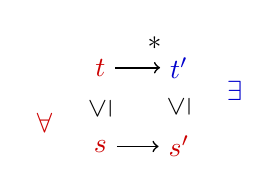
\begin{tikzpicture}[semithick, ->]
    \node[color=red!80!black] (s) {$s$};
    \node[color=red!80!black] (t) [above of=s] {$t$};
    \node[color=red!80!black] (sp) [right of=s] {$s'$};
    \node[color=blue!80!black] (tp) [right of=t] {$t'$};

    \path[color=white]  (s) edge node[color=black,rotate=90] {$\leq$} (t);
    \path  (s) edge (sp);
    \path  (t) edge node [above right] {*} (tp);
    \path[color=white]  (sp) edge node[color=black,rotate=90] {$\leq$} (tp);
    
    \node[color=blue!80!black] (exists) [above right of=sp] {$\exists$};
    \node[color=red!80!black] (forall) [below left of=t] {$\forall$};

    \end{tikzpicture}
    \end{center}
  \end{itemize}

  For more detail see: \cite{DBLP:journals/tcs/FinkelS01, DBLP:conf/lics/AbdullaCJT96}

\end{frame}

\begin{frame}
  \frametitle{Depth-bounded systems: \cite{Meyer08OnBoundednessInDepth}}
  System with a bound on the longest acyclic path.\\
  (Concretely: it is not possible to encode an infinite memory.)

  \vspace{10pt}

  \begin{figure}
  \centering
  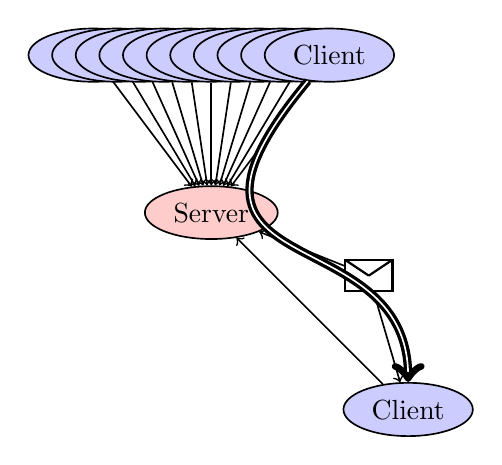
\begin{tikzpicture}[semithick, ->, node distance=2cm]
  \node [draw,ellipse,fill=red!20]  (x) at ( 0, 0) {Server};

  \node [draw,ellipse,fill=blue!20] (ni) at (-1.5, 2) {Client};
  \path  (ni) edge node [left] {} (x);
  \node [draw,ellipse,fill=blue!20] (n1) at (-1.2, 2) {Client};
  \path  (n1) edge (x);
  \node [draw,ellipse,fill=blue!20] (n2) at (-0.9, 2) {Client};
  \path  (n2) edge (x);
  \node [draw,ellipse,fill=blue!20] (n3) at (-0.6, 2) {Client};
  \path  (n3) edge (x);
  \node [draw,ellipse,fill=blue!20] (n4) at (-0.3, 2) {Client};
  \path  (n4) edge (x);
  \node [draw,ellipse,fill=blue!20] (n5) at ( 0  , 2) {Client};
  \path  (n5) edge (x);
  \node [draw,ellipse,fill=blue!20] (n6) at ( 0.3, 2) {Client};
  \path  (n6) edge (x);
  \node [draw,ellipse,fill=blue!20] (n7) at ( 0.6, 2) {Client};
  \path  (n7) edge (x);
  \node [draw,ellipse,fill=blue!20] (n8) at ( 0.9, 2) {Client};
  \path  (n8) edge (x);
  \node [draw,ellipse,fill=blue!20] (n9) at ( 1.2, 2) {Client};
  \path  (n9) edge (x);
  \node [draw,ellipse,fill=blue!20] (nj) at ( 1.5, 2) {Client};
  \path  (nj) edge node [left] {} (x);
  
  \node [draw,ellipse,fill=blue!20] (m) at ( 2.5, -2.5) {Client};
  \path  (m) edge node [below left] {} (x);
  
  \tikzMessageNode{mm}{2.0,-0.8}
  \path  (mm) edge node [right] {} (m);
  \path  (mm) edge node [above right] {} (x);

  \draw[very thick,double] (nj) .. controls (-1,-1) and (2.5,0) .. (m);

  \end{tikzpicture}
  \end{figure}
\end{frame}

\begin{frame}
  \frametitle{Why DBP are WSTS ?}

  \begin{description}
  \item[WQO] subgraph isomorphism for graphs of specific shapes (proof by a generalisation of Kruskal tree theorem).
  \item[Compatibility] The $\pi$-calculus has no fairness constraints. Additional processes (greater in the ordering) can simply be ignored.
  \end{description}
\end{frame}

\begin{frame}
  \frametitle{Backward algorithm for covering}
  \begin{center}
  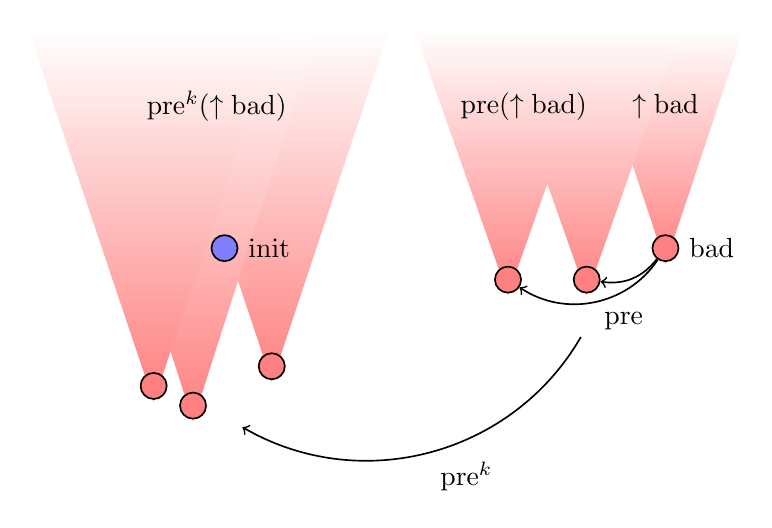
\begin{tikzpicture}[semithick,->]

  \shade[bottom color=red!50,top color=white] (3,5) -- (4,2) -- (5,5);
  \node[draw,circle,fill=red!50,minimum height=0.2,label={right:bad}] (e1) at (4,2.2) {};

  \visible<2->{
  \shade[bottom color=red!50,top color=white] (1.8,5) -- (3,1.6) -- (4.2,5);
  \node[draw,circle,fill=red!50,minimum height=0.2] (e2) at (3,1.8) {};
  \shade[bottom color=red!50,top color=white] (0.8,5) -- (2,1.6) -- (3.2,5);
  \node[draw,circle,fill=red!50,minimum height=0.2] (e3) at (2,1.8) {};
  \path (e1) edge[bend left] (e2);
  \path (e1) edge[bend left=45] node[below right] {pre} (e3);
  \node at (2.2,4) {$\text{pre}(\uparrow\text{bad})$};
  }

  \visible<3->{
  \shade[bottom color=red!50,top color=white] (-2.5,5) -- (-1,0.5) -- (0.5,5);
  \node[draw,circle,fill=red!50,minimum height=0.2] at (-1,0.7) {};
  \shade[bottom color=red!50,top color=white] (-3.6,5) -- (-2,0) -- (-0.4,5);
  \node[draw,circle,fill=red!50,minimum height=0.2] at (-2,0.2) {};
  \shade[bottom color=red!50,top color=white] (-4.1,5) -- (-2.5,0.25) -- (-0.9,5);
  \node[draw,circle,fill=red!50,minimum height=0.2] at (-2.5,0.45) {};

  \node (e4) at (3,1.2) {};
  \node (e5) at (-1.5,0) {};
  \path (e4) edge[bend left=45] node[below right] {pre$^k$} (e5);
  \node at (-1.7,4) {$\text{pre}^k(\uparrow\text{bad})$};
  }

  \visible<4->{
  \node[draw,circle,fill=blue!50,minimum height=0.2,label={right:init}] at (-1.6,2.2) {};
  }
  
  %on top of the shades
  \node at (4,4) {$\uparrow\text{bad}$};
  
  \end{tikzpicture}
  \end{center}

  \visible<5->{
  Computing the pre for DBP is not practical (aliasing problem)!\\
  Also the theoretical complexity is terrible.
  }

\end{frame}

\begin{frame}
  \frametitle{Forward algorithm for covering using acceleration}
  \begin{center}
  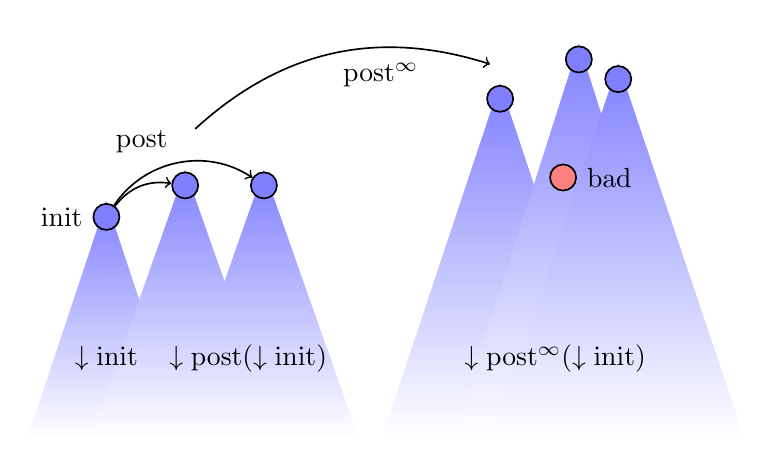
\begin{tikzpicture}[semithick,->]

  \shade[top color=blue!50,bottom color=white] (-3,-5) -- (-4,-2) -- (-5,-5);
  \node[draw,circle,fill=blue!50,minimum height=0.2,label={left:init}] (e1) at (-4,-2.2) {};

  \visible<2->{
  \shade[top color=blue!50,bottom color=white] (-1.8,-5) -- (-3,-1.6) -- (-4.2,-5);
  \node[draw,circle,fill=blue!50,minimum height=0.2] (e2) at (-3,-1.8) {};
  \shade[top color=blue!50,bottom color=white] (-0.8,-5) -- (-2,-1.6) -- (-3.2,-5);
  \node[draw,circle,fill=blue!50,minimum height=0.2] (e3) at (-2,-1.8) {};
  \path (e1) edge[bend left] (e2);
  \path (e1) edge[bend left=45] node[above left] {post} (e3);
  \node at (-2.2,-4) {$\downarrow\text{post}(\downarrow\text{init})$};
  }

  \visible<3->{
  \shade[top color=blue!50,bottom color=white] (2.5,-5) -- (1,-0.5) -- (-0.5,-5);
  \node[draw,circle,fill=blue!50,minimum height=0.2] at (1,-0.7) {};
  \shade[top color=blue!50,bottom color=white] (3.6,-5) -- (2,0) -- (0.4,-5);
  \node[draw,circle,fill=blue!50,minimum height=0.2] at (2,-0.2) {};
  \shade[top color=blue!50,bottom color=white] (4.1,-5) -- (2.5,-0.25) -- (0.9,-5);
  \node[draw,circle,fill=blue!50,minimum height=0.2] at (2.5,-0.45) {};

  \node (e4) at (-3,-1.2) {};
  \node (e5) at (1,-0.3) {};
  \path (e4) edge[bend left] node[below right] {post$^\infty$} (e5);
  \node at (1.7,-4) {$\downarrow\text{post}^\infty(\downarrow\text{init})$};
  }

  \visible<4->{
  \node[draw,circle,fill=red!50,minimum height=0.2,label={right:bad}] at (1.8,-1.7) {};
  }
  %on top of the shades
  \node at (-4,-4) {$\downarrow\text{init}$};
  \end{tikzpicture}
  \end{center}
  
  \visible<5->{
  Successfully applied to Petri nets (+extensions) and lossy channels systems.
  Even though computing the covering set is not decidable \cite{DBLP:conf/icalp/DufourdFS98}.
  }
\end{frame}

\begin{frame}
  \frametitle{Adequate domain of limits}
  ADL: \cite{GeeraertsETAL06ExpandEnlargeCheck}\\
  Further developed in \cite{FinkelGoubaultLarrecq09ForwardAnalysisForWSTS}\\
  Applied to DBP in \cite{WiesETAL10ForwardAnalysisofDepthBoundedProcesses}

  \begin{figure}
  \centering
  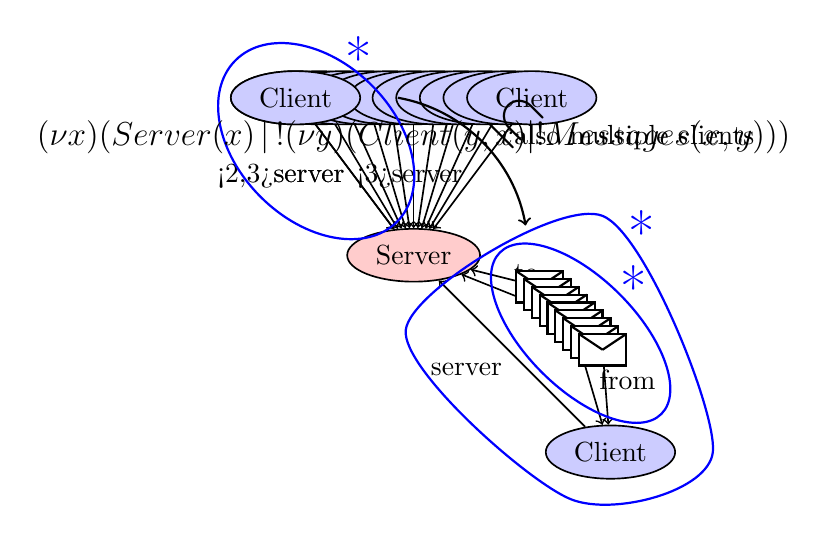
\begin{tikzpicture}[semithick, ->, node distance=2cm]
  \node [draw,ellipse,fill=red!20]  (x) at ( 0, 0) {Server};

  %replication of clients
  \visible<2-4> {
  \node [draw,ellipse,fill=blue!20] (ni) at (-1.5, 2) {Client};
  \path  (ni) edge node [left] {\alt<2,3>{server}{}} (x);
  }

  \visible<4> {
  \node [draw,ellipse,fill=blue!20] (n1) at (-1.2, 2) {Client};
  \path  (n1) edge (x);
  \node [draw,ellipse,fill=blue!20] (n2) at (-0.9, 2) {Client};
  \path  (n2) edge (x);
  \node [draw,ellipse,fill=blue!20] (n3) at (-0.6, 2) {Client};
  \path  (n3) edge (x);
  \node [draw,ellipse,fill=blue!20] (n4) at (-0.3, 2) {Client};
  \path  (n4) edge (x);
  \node [draw,ellipse,fill=blue!20] (n5) at ( 0  , 2) {Client};
  \path  (n5) edge (x);
  \node [draw,ellipse,fill=blue!20] (n6) at ( 0.3, 2) {Client};
  \path  (n6) edge (x);
  \node [draw,ellipse,fill=blue!20] (n7) at ( 0.6, 2) {Client};
  \path  (n7) edge (x);
  \node [draw,ellipse,fill=blue!20] (n8) at ( 0.9, 2) {Client};
  \path  (n8) edge (x);
  \node [draw,ellipse,fill=blue!20] (n9) at ( 1.2, 2) {Client};
  \path  (n9) edge (x);
  }

  \visible<3-4> {
  \node [draw,ellipse,fill=blue!20] (nj) at ( 1.5, 2) {Client};
  \path  (nj) edge node [left] {\alt<3>{server}{}} (x);
  }
  
  \visible<5-12> {
  \node [draw,ellipse,fill=blue!20] (n) at ( -1.5, 2) {Client};
  \path  (n) edge node [left] {server} (x);
  \draw[thick,rotate=45,color=blue] (0.15,1.9) ellipse (1 and 1.45);
  \node[text=blue] (star) at ( -0.7, 2.5) {{\huge *}};
  }
  
  %replication of messages
  \visible<6-> {
  \node [draw,ellipse,fill=blue!20] (m) at ( 2.5, -2.5) {Client};
  \path  (m) edge node [below left] {server} (x);
  }
  
  \visible<7,9-> {
  \tikzMessageNode{mm}{2.0,-0.8}
  \path  (mm) edge node [right] {from} (m);
  \path  (mm) edge node [above right] {to} (x);
  }

  \visible<8> {
  \tikzMessageNode{m1}{1.6,-0.4}
  \tikzMessageNode{m3}{1.7,-0.5}
  \tikzMessageNode{m4}{1.8,-0.6}
  \tikzMessageNode{m5}{1.9,-0.7}
  \tikzMessageNode{m6}{2.0,-0.8}
  \tikzMessageNode{m7}{2.1,-0.9}
  \tikzMessageNode{m8}{2.2,-1.0}
  \tikzMessageNode{m9}{2.3,-1.1}
  \tikzMessageNode{m2}{2.4,-1.2}
  \path  (m2) edge (m);
  \path  (m1) edge (x);
  }

  \visible<9-> {
  \draw[thick,rotate=45,color=blue] (0.8,-2.2) ellipse (0.7 and 1.45);
  \node[text=blue] (star) at ( 2.8, -0.4) {{\huge *}};
  }

  \visible<10-12> {
  \draw[thick] (-.2,2) arc (80:10:2);
  }
  \visible<10> {
  \node (txt1) at ( 2.8, 1.5) {also multiple clients};
  }
  \visible<12> {
  \node[rotate=-45] (txt2) at ( 1.3, 1.7) {{\huge $\subseteq$}};
  }
  
  \visible<11-> {
  \draw[color=blue,thick] plot[smooth cycle] coordinates{(-0.1,-0.95) (2.4,0.5) (3.8,-2.5) (2,-3.1)};
  \node[text=blue] (star) at ( 2.9, 0.3) {{\huge *}};
  }

  \visible<14> {
  \node at (0,1.5) {{\large $(\nu x)(Server(x) \,|\, !(\nu y)(Client(y,x) | !Messages(x,y)))$}};
  }

  \end{tikzpicture}
  \end{figure}
\end{frame}

\begin{frame}
  \frametitle{When does acceleration work ? (flat systems)}

  Usually forward algorithms are based on acceleration.
  By acceleration we mean computing the result of executing a loop infinitely many time.

  \vspace{10pt}

  We can see this as computing the result of execution traces of length $< \omega^2$.
  Concretely, it means that the algorithm can saturate the covering set by executing only simple loops (see \cite{DBLP:conf/atva/BardinFLS05}).
  This condition is known as flattability.


  
  \begin{figure}
  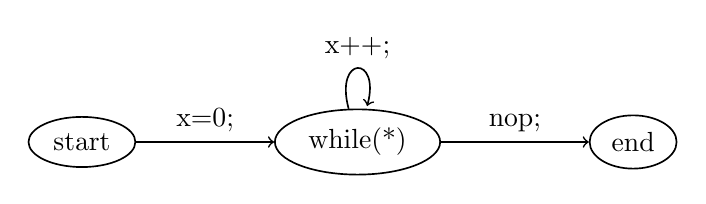
\begin{tikzpicture}[semithick, ->, node distance=35mm]

  \node [draw,ellipse] (loc1) at ( 0, 0) {start};
  \node [draw,ellipse] (loc2) [right of=loc1] {while(*)};
  \node [draw,ellipse] (loc3) [right of=loc2] {end};
  \path  (loc1) edge node[above] {x=0;} (loc2);
  \path  (loc2) edge [loop above] node[above] {x++;}(loc2);
  \path  (loc2) edge node[above] {nop;} (loc3);
  \end{tikzpicture}
  \caption{Example of a flat program}
  \end{figure}

\end{frame}

\begin{frame}
  \frametitle{DBP are intrinsically not flat.}

  \begin{minipage}{0.6\linewidth}
  initial configuration:
  
  \begin{figure}
  \centering
  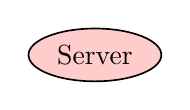
\begin{tikzpicture}[semithick, ->, node distance=2cm]
  \node [draw,ellipse,fill=red!20]  (x) at ( 0, 0) {Server};
  \end{tikzpicture}
  \end{figure}

  covering set:

  \begin{figure}
  \centering
  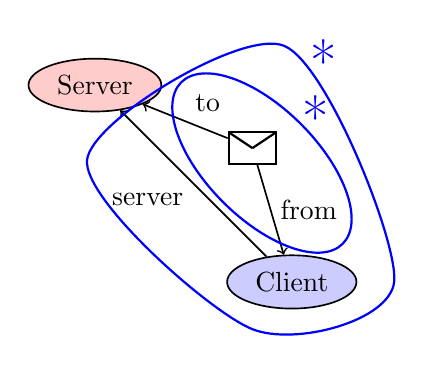
\begin{tikzpicture}[semithick, ->, node distance=2cm]
  \node [draw,ellipse,fill=red!20]  (x) at ( 0, 0) {Server};

  \node [draw,ellipse,fill=blue!20] (m) at ( 2.5, -2.5) {Client};
  \path  (m) edge node [below left] {server} (x);
  
  \tikzMessageNode{mm}{2.0,-0.8}
  \path  (mm) edge node [right] {from} (m);
  \path  (mm) edge node [above right] {to} (x);

  \draw[thick,rotate=45,color=blue] (0.8,-2.2) ellipse (0.7 and 1.45);
  \node[text=blue] (star) at ( 2.8, -0.4) {{\huge *}};

  \draw[color=blue,thick] plot[smooth cycle] coordinates{(-0.1,-0.95) (2.4,0.5) (3.8,-2.5) (2,-3.1)};
  \node[text=blue] (star) at ( 2.9, 0.3) {{\huge *}};

  \end{tikzpicture}
  \end{figure}
  
  \end{minipage}
  \begin{minipage}{0.35\linewidth}
  How many steps are there between the initial configuration and the final configuration ?

  $\omega^2$ steps

  \vspace{10pt}

  Hence, we need to consider nested loops if we want to compute the covering set.
  \end{minipage}

\end{frame}

\begin{frame}
  \frametitle{From acceleration to widening}

  Acceleration considers transitions.
  Widening only states.

  \begin{figure}
  \centering
  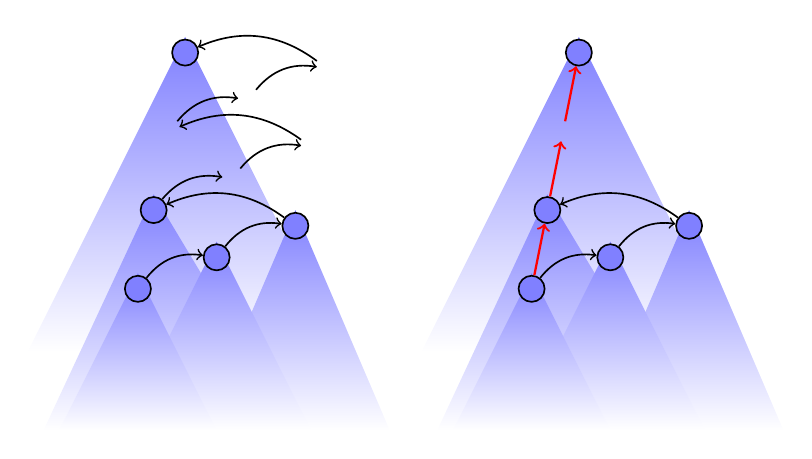
\begin{tikzpicture}[semithick, ->, node distance=2cm]

  \begin{scope}
  
  %layer 1: shades
  \visible<6->{
    \shade[top color=blue!50,bottom color=white] (-1.4,-3) -- (-3.4,1) -- (-5.4,-3);
  }
  \visible<5->{
  }
  \visible<4->{
    \shade[top color=blue!50,bottom color=white] (-2,-4) -- (-3.8,-1.0) -- (-5.2,-4);
  }
  \visible<3->{
    \shade[top color=blue!50,bottom color=white] (-0.8,-4) -- (-2,-1.2) -- (-3.2,-4);
  }
  \visible<2->{
    \shade[top color=blue!50,bottom color=white] (-1.8,-4) -- (-3,-1.6) -- (-4.2,-4);
  }
  \visible<1->{
    \shade[top color=blue!50,bottom color=white] (-3,-4) -- (-4,-2) -- (-5,-4);
  }
  
  %layer 2: nodes
  \visible<1->{
    \node[draw,circle,fill=blue!50] (e1) at (-4,-2.2) {};
  }
  \visible<2->{
    \node[draw,circle,fill=blue!50] (e2) at (-3,-1.8) {};
  }
  \visible<3->{
    \node[draw,circle,fill=blue!50] (e3) at (-2,-1.4) {};
  }
  \visible<4->{
    \node[draw,circle,fill=blue!50] (e4) at (-3.8,-1.2) {};
  }
  \visible<5->{
    \node (e5) at (-2.8,-0.8) {};
    \node (e6) at (-1.8,-0.4) {};
    \node (e7) at (-3.6,-0.2) {};
  }
  \visible<6->{
    \node (e8) at (-2.6,0.2) {};
    \node (e9) at (-1.6,0.6) {};
    \node[draw,circle,fill=blue!50] (e10) at (-3.4,0.8) {};
  }

  %layer 3: edges 
  \visible<1->{
  }
  \visible<2->{
    \path (e1) edge[bend left] (e2);
  }
  \visible<3->{
    \path (e2) edge[bend left] (e3);
  }
  \visible<4->{
    \path (e3) edge[bend right] (e4);
  }
  \visible<5->{
    \path (e4) edge[bend left] (e5);
    \path (e5) edge[bend left] (e6);
    \path (e6) edge[bend right] (e7);
  }
  \visible<6->{
    \path (e7) edge[bend left] (e8);
    \path (e8) edge[bend left] (e9);
    \path (e9) edge[bend right] (e10);
  }
  
  \end{scope}
  
  \begin{scope}[xshift=5cm]
  
  %layer 1: shades
  \visible<12->{
    \shade[top color=blue!50,bottom color=white] (-1.4,-3) -- (-3.4,1) -- (-5.4,-3);
  }
  \visible<11->{
  }
  \visible<10->{
    \shade[top color=blue!50,bottom color=white] (-2,-4) -- (-3.8,-1.0) -- (-5.2,-4);
  }
  \visible<9->{
    \shade[top color=blue!50,bottom color=white] (-0.8,-4) -- (-2,-1.2) -- (-3.2,-4);
  }
  \visible<8->{
    \shade[top color=blue!50,bottom color=white] (-1.8,-4) -- (-3,-1.6) -- (-4.2,-4);
  }
  \visible<7->{
    \shade[top color=blue!50,bottom color=white] (-3,-4) -- (-4,-2) -- (-5,-4);
  }
  
  %layer 2: nodes
  \visible<7->{
    \node[draw,circle,fill=blue!50] (e1) at (-4,-2.2) {};
  }
  \visible<8->{
    \node[draw,circle,fill=blue!50] (e2) at (-3,-1.8) {};
  }
  \visible<9->{
    \node[draw,circle,fill=blue!50] (e3) at (-2,-1.4) {};
  }
  \visible<10->{
    \node[draw,circle,fill=blue!50] (e4) at (-3.8,-1.2) {};
  }
  \visible<11->{
  }
  \visible<12->{
    \node (e7) at (-3.6,-0.2) {};
    \node[draw,circle,fill=blue!50] (e10) at (-3.4,0.8) {};
  }

  %layer 3: edges 
  \visible<7->{
  }
  \visible<8->{
    \path (e1) edge[bend left] (e2);
  }
  \visible<9->{
    \path (e2) edge[bend left] (e3);
  }
  \visible<10->{
    \path (e3) edge[bend right] (e4);
  }
  \visible<11->{
    \path (e1) edge[red,thick] (e4);
  }
  \visible<12->{
    \path (e4) edge[red,thick] (e7);
    \path (e7) edge[red,thick] (e10);
  }
  
  \end{scope}

  \end{tikzpicture}
  \end{figure}

\end{frame}

% TODO a bit of formalism, The VMCAI thing.

\begin{frame}
  \frametitle{Abstract interpretation: Domains}

  \begin{itemize}
  \item Concrete domain: $D = \mathcal{P}(S)$
  \item Abstract domain: $D_\downarrow = \{\ \downarrow X ~ | ~ X \subseteq S \}$
  \end{itemize}
  
  The abstract domain can be further refined from the set of downward-closed set to the set of ideals (downward-closed and \emph{directed}).

  \begin{itemize}
  \item Abstract domain 2: $D_{\mathit{Idl}}$
  \end{itemize}

  An arbitray downward-closed set can be represented as the finite union of ideals.

\end{frame}

\begin{frame}
  \frametitle{Widening (1)}

  Goal: try to mimic acceleration (when possible), and force termination
  
  \vspace{1ex}

  A set-widening operator ($\nabla$) for a poset $X$ is partial function ($\mathcal{P}(X) \rightarrow X$) that satisfies:
  \begin{description}
  \item[Covering]: for all $Y \subseteq X$, $y \in Y \Rightarrow y \leq \nabla(Y)$;
  \item[Termination]: widening of any ascending chain stabilizes.
  \end{description}

  \vspace{1ex}

  Reason of using a set-widening operator: we need the history.

\end{frame}

\begin{frame}
  \frametitle{Widening (2)}

  Lifting a widening operators from $\mathit{Idl}(S)$ to $D_{\mathit{Idl}}$:
  going from elements of the domain to finite powerset is non-trivial.
  We assume that the ordering is a \emph{bqo}.
  Thus $\mathit{Idl}(S)$ is also a bqo.

  \vspace{1ex}
  
  Given an ascending chain: $C = \{L_i\}_{0 \leq i \leq n}, C \subseteq D_{\mathit{Idl}}$ (history)
  \begin{itemize}
  \item $\nabla(\{L_0\}) = \{L_0\}$
  \item $\nabla(\{L_0, \ldots, L_i\}) = \nabla(\{L_0, \ldots, L_{i-1}\}) \sqcup \{\nabla_S(\mathcal{I})\ ~|~ \mathcal{I} ~ \text{max ascending chain in} \nabla(\{L_0, \ldots, L_{i-1}\})\}$
  \end{itemize}

  \vspace{1ex}

  Why a \emph{bqo} ? 
  To avoid having an infinite antichain in $\mathit{Idl}(S)$.


\end{frame}

\begin{frame}
  \frametitle{Set-widening for DBP (1)}

  \begin{figure}
  \centering
  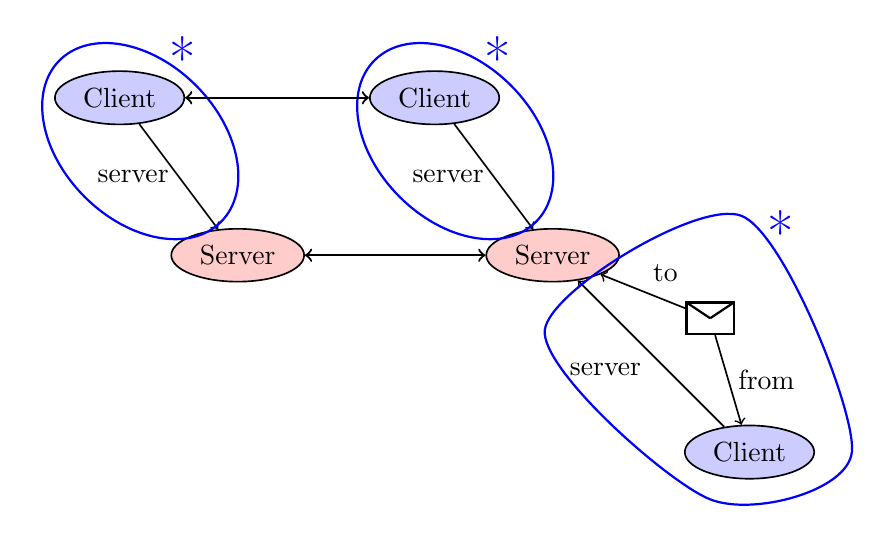
\begin{tikzpicture}[semithick, ->, node distance=2cm]


  \begin{scope}
    \node [draw,ellipse,fill=red!20]  (x) at ( 0, 0) {Server};
    \node [draw,ellipse,fill=blue!20] (ni) at (-1.5, 2) {Client};
    \path  (ni) edge node [left] {server} (x);
    \draw[thick,rotate=45,color=blue] (0.15,1.9) ellipse (1 and 1.45);
    \node[text=blue] (star) at ( -0.7, 2.5) {{\huge *}};
  \end{scope}
  
  \begin{scope}[xshift=4cm]
    \node [draw,ellipse,fill=red!20]  (x2) at ( 0, 0) {Server};
    \node [draw,ellipse,fill=blue!20] (ni2) at (-1.5, 2) {Client};
    \path  (ni2) edge node [left] {server} (x2);
    \draw[thick,rotate=45,color=blue] (0.15,1.9) ellipse (1 and 1.45);
    \node[text=blue] (star) at ( -0.7, 2.5) {{\huge *}};
    \node [draw,ellipse,fill=blue!20] (m) at ( 2.5, -2.5) {Client};
    \path  (m) edge node [below left] {server} (x2);
    \tikzMessageNode{mm}{2.0,-0.8}
    \path  (mm) edge node [right] {from} (m);
    \path  (mm) edge node [above right] {to} (x2);
  \end{scope}
  
  \visible<2->{
    \path[<->,thick] (x) edge (x2);
    \path[<->,thick] (ni) edge (ni2);
  }
  \visible<3->{
    \draw[color=blue,thick] plot[smooth cycle] coordinates{(3.9,-0.95) (6.4,0.5) (7.8,-2.5) (6,-3.1)};
    \node[text=blue] (star) at ( 6.9, 0.3) {{\huge *}};
  }

  \end{tikzpicture}
  \end{figure}
\end{frame}

\begin{frame}
  \frametitle{Set-widening for DBP (2)}

  \begin{figure}
  \centering
  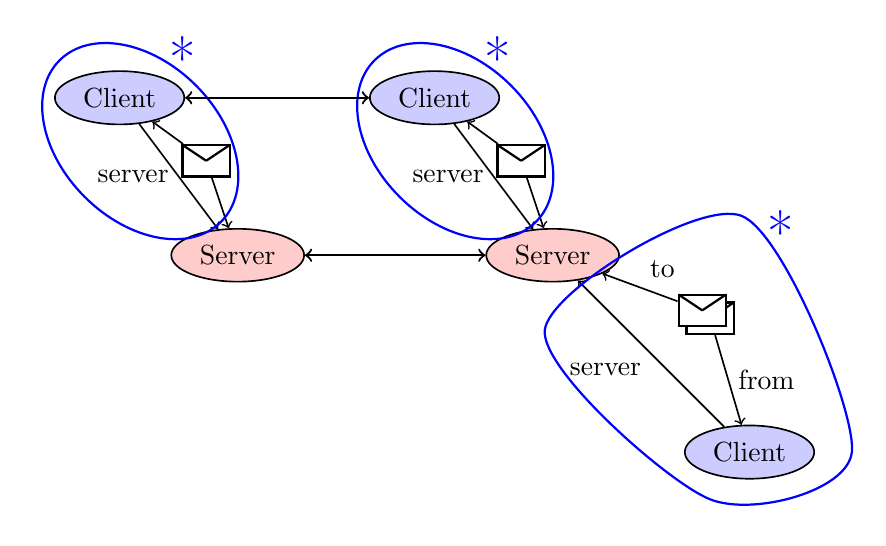
\begin{tikzpicture}[semithick, ->, node distance=2cm]

  \begin{scope}
    \node [draw,ellipse,fill=red!20]  (x) at ( 0, 0) {Server};
    \node [draw,ellipse,fill=blue!20] (ni) at (-1.5, 2) {Client};
    \path  (ni) edge node [left] {server} (x);
    \tikzMessageNode{om}{-0.4,1.2}
    \path  (om) edge (x);
    \path  (om) edge (ni);
    \draw[thick,rotate=45,color=blue] (0.15,1.9) ellipse (1 and 1.45);
    \node[text=blue] (star) at ( -0.7, 2.5) {{\huge *}};
  \end{scope}
  
  \begin{scope}[xshift=4cm]
    \node [draw,ellipse,fill=red!20]  (x2) at ( 0, 0) {Server};
    \node [draw,ellipse,fill=blue!20] (ni2) at (-1.5, 2) {Client};
    \path  (ni2) edge node [left] {server} (x2);
    \tikzMessageNode{om2}{-0.4,1.2}
    \path  (om2) edge (x2);
    \path  (om2) edge (ni2);
    \draw[thick,rotate=45,color=blue] (0.15,1.9) ellipse (1 and 1.45);
    \node[text=blue] (star) at ( -0.7, 2.5) {{\huge *}};
    \node [draw,ellipse,fill=blue!20] (m) at ( 2.5, -2.5) {Client};
    \path  (m) edge node [below left] {server} (x2);
    \tikzMessageNode{mm}{2.0,-0.8}
    \tikzMessageNode{mm2}{1.9,-0.7}
    \path  (mm) edge node [right] {from} (m);
    \path  (mm2) edge node [above right] {to} (x2);
  \end{scope}
  
  \visible<2->{
    \path[<->,thick] (x) edge (x2);
    \path[<->,thick] (ni) edge (ni2);
  }
  \visible<3->{
    \draw[color=blue,thick] plot[smooth cycle] coordinates{(3.9,-0.95) (6.4,0.5) (7.8,-2.5) (6,-3.1)};
    \node[text=blue] (star) at ( 6.9, 0.3) {{\huge *}};
  }

  \end{tikzpicture}
  \end{figure}
\end{frame}

\begin{frame}
  \frametitle{Set-widening for DBP (3)}

  \begin{figure}
  \centering
  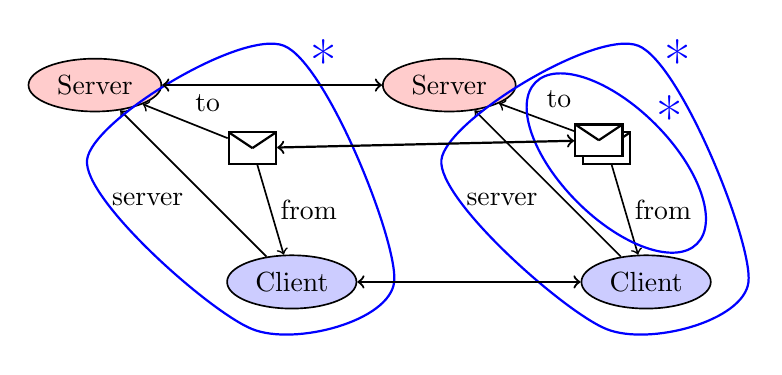
\begin{tikzpicture}[semithick, ->, node distance=2cm]

  \visible<2->{
  \begin{scope}
    \node [draw,ellipse,fill=red!20]  (x) at ( 0, 0) {Server};
    \node [draw,ellipse,fill=blue!20] (m) at ( 2.5, -2.5) {Client};
    \path  (m) edge node [below left] {server} (x);
    \tikzMessageNode{mm}{2.0,-0.8}
    \path  (mm) edge node [right] {from} (m);
    \path  (mm) edge node [above right] {to} (x);
    \draw[color=blue,thick] plot[smooth cycle] coordinates{(-0.1,-0.95) (2.4,0.5) (3.8,-2.5) (2,-3.1)};
    \node[text=blue] (star) at ( 2.9, 0.3) {{\huge *}};
  \end{scope}
  }
  
  \begin{scope}[xshift=4.5cm]
    \node [draw,ellipse,fill=red!20]  (x2) at ( 0, 0) {Server};
    \node [draw,ellipse,fill=blue!20] (m2) at ( 2.5, -2.5) {Client};
    \path  (m2) edge node [below left] {server} (x2);
    \tikzMessageNode{mm1}{2.0,-0.8}
    \tikzMessageNode{mm2}{1.9,-0.7}
    \path  (mm1) edge node [right] {from} (m2);
    \path  (mm2) edge node [above right] {to} (x2);
    \draw[color=blue,thick] plot[smooth cycle] coordinates{(-0.1,-0.95) (2.4,0.5) (3.8,-2.5) (2,-3.1)};
    \node[text=blue] (star) at ( 2.9, 0.3) {{\huge *}};
    \visible<4->{
      \draw[thick,rotate=45,color=blue] (0.8,-2.2) ellipse (0.7 and 1.45);
      \node[text=blue] (star) at ( 2.8, -0.4) {{\huge *}};
    }
  \end{scope}
  
  \visible<3->{
    \path[<->,thick] (x) edge (x2);
    \path[<->,thick] (m) edge (m2);
    \path[<->,thick] (mm) edge (mm2);
  }

  \end{tikzpicture}
  \end{figure}
\end{frame}

\iffalse
\begin{frame}
  \frametitle{Termination of the analysis}

  \begin{itemize}
  \item Wqo is not enough, we also need a bqo.
  \item Our system is depth-bounded. The widening adds some ``!'' in the formula describing the configuration.
  \item We also keep the whole history for the widening (more than pairwise widening).
  %\item By messing around with the congruence relation, the fact that the covering problem is upward-closed and some other property
  \end{itemize}
  
\end{frame}
\fi

\begin{frame}
  \frametitle{What about the precision ?}

  \begin{itemize}
  \item Acceleration and widening seems like the \emph{extreme} ends of some spectrum.
  \item Is there a class of nested loops for which we can compute exactly the result ?
  \item Can we get a good characterisation of the programs for which this kind of widening matches acceleration ?
  \end{itemize}

\end{frame}

\begin{frame}
  \frametitle{Recap}

  \begin{itemize}
  \item DBP is one of the largest fragment of the $\pi$-calculus for which interesting verification questions are still decidable.
  \item Not yet clear what is the right way of handling features such as process creation and mobility.
  \item WSTS approach gives decidability a result, now we are working on an efficient analysis.
  \end{itemize}

\end{frame}

\begin{frame}
  \frametitle{}
  \begin{center}
  {\Large Questions ?}
  \end{center}
\end{frame}

\begin{frame}[allowframebreaks]{References}
  \frametitle{}
  {\tiny
  %\bibliographystyle{annotate}
  %\bibliographystyle{plainnat}
  \bibliographystyle{cell}
  %\bibliographystyle{abbrvnat}
  \bibliography{biblio}
  }
\end{frame}

\end{document}
